\documentclass{article}
\usepackage{graphicx} % Required for inserting images
\usepackage{float}
\usepackage{placeins}  % for \FloatBarrier to stop floats wandering
\usepackage{caption}   % for \captionof inside minipage
\usepackage{amsmath}
\usepackage{listings}
\usepackage{steinmetz} % for A\angle\phi notation
\usepackage{siunitx}   % for units like \SI{50}{\ohm}
\usepackage{amssymb, amsfonts}
\usepackage{booktabs}  % for nice tables
\usepackage{physics}   % for \dv, \abs, etc.
\usepackage[margin=2.2cm]{geometry}
\lstset{
  language=Matlab,
  basicstyle=\ttfamily\small,
  keywordstyle=\bfseries,
  commentstyle=\itshape,
  numbers=left,
  numbersep=6pt,
  stepnumber=1,
  frame=single,
  breaklines=true,
  showstringspaces=false,
  columns=fullflexible,
  keepspaces=true,
  xleftmargin=2mm
}
\newcommand{\ang}[1]{\,\angle\,#1^{\circ}}


\title{Week 2}
\author{Ahmad Al kadi}
\date{October 2025}

\begin{document}

\maketitle

\section{Introduction}



\section*{Exercise 1: From Sinusoids to Phasors \quad }

\textbf{Given data}

\[
\begin{aligned}
v_{1}(t) &= 200\,\sin(\omega t-60^\circ)\ \text{V},\\
v_{2}(t) &= 150\,\sin(\omega t+90^\circ)\ \text{V},\\
i(t)     &= 8\,\cos(\omega t+120^\circ)\ \text{A},\\
\omega   &= 628\ \text{rad·s}^{-1},\\
f        &= \dfrac{\omega}{2\pi}\approx 100\ \text{Hz}.
\end{aligned}
\]


% ==================================================
\subsection*{1. Time to phasor conversion}
% ==================================================

We use \emph{cosine} as the reference waveform.  
Identity: \(\sin x=\cos(x-90^\circ)\).  
A cosine \(A\cos(\omega t+\phi)\) maps to the phasor \(A\angle\phi\).

\[
\begin{aligned}
v_1(t) &= 200\sin(\omega t-60^\circ)
       = 200\cos(\omega t-150^\circ)\\
       &\Rightarrow V_1 = 200\angle(-150^\circ)\ \text{V}
\end{aligned}
\]

\[
\begin{aligned}
v_2(t) &= 150\sin(\omega t+90^\circ)
       = 150\cos(\omega t+0^\circ)\\
       &\Rightarrow V_2 = 150\angle(0^\circ)\ \text{V}
\end{aligned}
\]

\[
\begin{aligned}
i(t) &= 8\cos(\omega t+120^\circ)\\
     &\Rightarrow I = 8\angle(120^\circ)\ \text{A}
\end{aligned}
\]

These transformations follow \emph{Mono.pdf}, sections 2.4 – 2.5.

% ==================================================
\subsection*{2. Phasor addition of \(v_1\) and \(v_2\)}
% ==================================================

Convert each to rectangular form:

\[
\begin{aligned}
V_1 &= 200(\cos(-150^\circ)+j\sin(-150^\circ))\\
    &= -173.2051 - j100.0000\ \text{V}
\end{aligned}
\]

\[
\begin{aligned}
V_2 &= 150(\cos 0^\circ + j\sin 0^\circ)\\
    &= 150 + j0\ \text{V}
\end{aligned}
\]

Add them:

\[
\begin{aligned}
V_{\text{sum}} &= V_1 + V_2\\
               &= (-23.2051 - j100.0000)\ \text{V}
\end{aligned}
\]

Compute magnitude and phase:

\[
\begin{aligned}
|V_{\text{sum}}|
 &= \sqrt{(-23.2051)^2 + (-100.0000)^2}\\
 &= 102.657\ \text{V}
\end{aligned}
\]

\[
\begin{aligned}
\angle V_{\text{sum}}
 &= \tan^{-1}\!\left(\frac{-100.0000}{-23.2051}\right)\\
 &= -103.064^\circ
\end{aligned}
\]

\[
\boxed{v_1(t)+v_2(t)=102.657\cos(\omega t-103.064^\circ)\ \text{V}}
\]

% ==================================================
\subsection*{3. Instantaneous and average power}
% ==================================================

\[
\begin{aligned}
p(t)
 &= 200\sin(\omega t-60^\circ)\cdot8\cos(\omega t+120^\circ)\\
 &= 1600\sin A\cos B
  = 800[\sin(A+B)+\sin(A-B)]
\end{aligned}
\]

where \(A=\omega t-60^\circ\), \(B=\omega t+120^\circ\).

\[
A+B=2\omega t+60^\circ,\qquad A-B=-180^\circ
\]

\[
\boxed{p(t)=800\,\sin(2\omega t+60^\circ)\ \text{W}}
\]

The average over one period is zero.  
Verification with RMS values:

\[
\begin{aligned}
P_{\text{avg}}
 &= V_{\text{rms}}I_{\text{rms}}\cos\phi\\
 &= \frac{200}{\sqrt2}\frac{8}{\sqrt2}\cos90^\circ = 0\ \text{W}
\end{aligned}
\]

% ==================================================
\subsection*{4. Effect of doubling the frequency}
% ==================================================

For \(\omega' = 2\omega\):

\[
\begin{aligned}
p'(t)
 &= 800\,\sin(2\omega' t + 60^\circ)\\
 &= 800\,\sin(4\omega t + 60^\circ)
\end{aligned}
\]

Thus the ripple frequency doubles, while phasors \(V_1\), \(V_2\), \(I\), and \(V_{\text{sum}}\) remain unchanged.


\subsection*{MATLAB}

The following MATLAB script verifies the analytical results by plotting
the three time–domain signals and their sum over one period:

\begin{verbatim}
% MATLAB Verification for Exercise 1 - Variant C

clear; clc;

% Given data
w = 628;           % rad/s
t = 0:1e-4:0.02;   % time vector (0–20 ms, one period)
v1 = 200*sin(w*t - deg2rad(60));
v2 = 150*sin(w*t + deg2rad(90));
i  = 8*cos(w*t + deg2rad(120));

% Phasor addition (check result)
v_sum = v1 + v2;

% Plot results
figure;
plot(t, v1, 'r', 'LineWidth', 1.2); hold on;
plot(t, v2, 'b', 'LineWidth', 1.2);
plot(t, v_sum, 'k', 'LineWidth', 1.4);
xlabel('Time (s)');
ylabel('Voltage (V)');
title('v1(t), v2(t), and v1(t)+v2(t)');
legend('v1(t)', 'v2(t)', 'v1(t)+v2(t)');
grid on;

% Instantaneous power (for v1 and i)
p = v1 .* i;
figure;
plot(t, p, 'm', 'LineWidth', 1.2);
xlabel('Time (s)');
ylabel('Power (W)');
title('Instantaneous Power p(t) = v1(t) * i(t)');
grid on;
\end{verbatim}

The plots confirm:
\begin{itemize}
\item The sum \(v_1(t)+v_2(t)\) matches the amplitude and phase 
      obtained analytically (\(102.657\angle -103.064^\circ\)).
\item The instantaneous power \(p(t)\) oscillates around zero, as predicted.
\end{itemize}


\begin{figure}[H]
\centering
\includegraphics[width=0.8\textwidth]{voltages (Ex 1).png}
\caption{Voltages $v_1(t)$, $v_2(t)$, and their sum $v_1(t)+v_2(t)$}
\end{figure}

\begin{figure}[H]
\centering
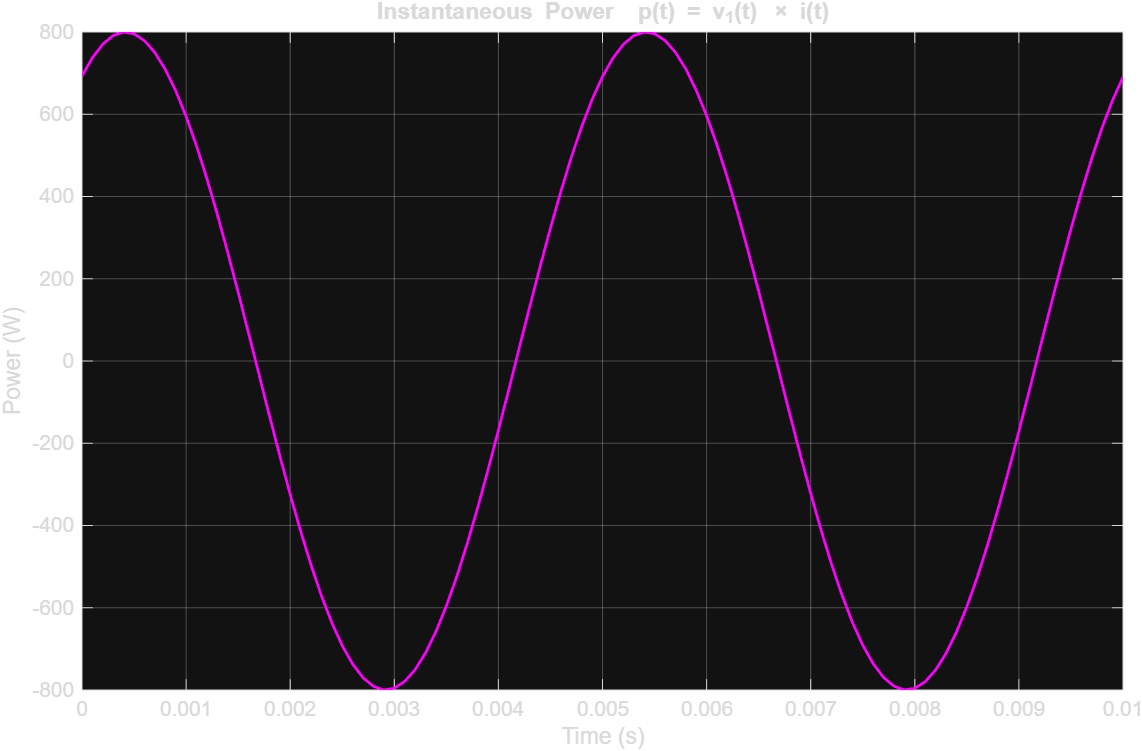
\includegraphics[width=0.8\textwidth]{Instantaneous Power (Ex 1).png}
\caption{Instantaneous power $p(t) = v_1(t) \cdot i(t)$}
\end{figure}



\section*{Technology Deliverables}

\subsection*{1. Web-based phasor calculator (HTML/JavaScript)}
A single-file HTML/JavaScript tool that computes the sum of two phasors.
Inputs are magnitude and angle (degrees). The script converts to rectangular
form, adds components, converts back to polar, and also prints the cosine
time-domain form. A small canvas draws \(V_1\), \(V_2\), and \(V_{\text{sum}}\).

\begin{figure}[H]
  \centering
  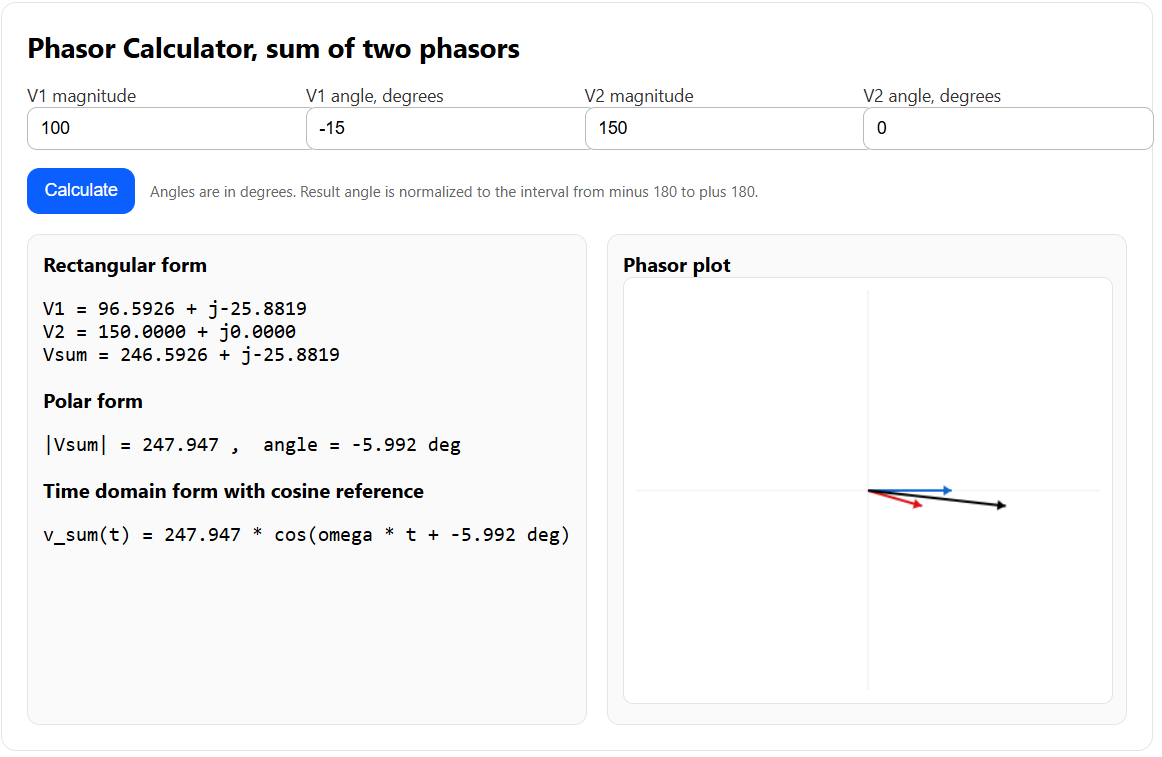
\includegraphics[width=\textwidth]{phasor_calculator.png}
  \caption{Web-based phasor calculator (HTML/JavaScript).}
\end{figure}

\subsection*{2. Animated GIF showing phasor addition}
The following animation was generated in MATLAB using the script
\texttt{make\_phasor\_gif.m}. It visualizes the head-to-tail addition of two
sinusoidal voltages represented as rotating phasors. The resulting black vector
shows the instantaneous sum of \( V_1 \) and \( V_2 \).

\begin{figure}[H]
    \centering
    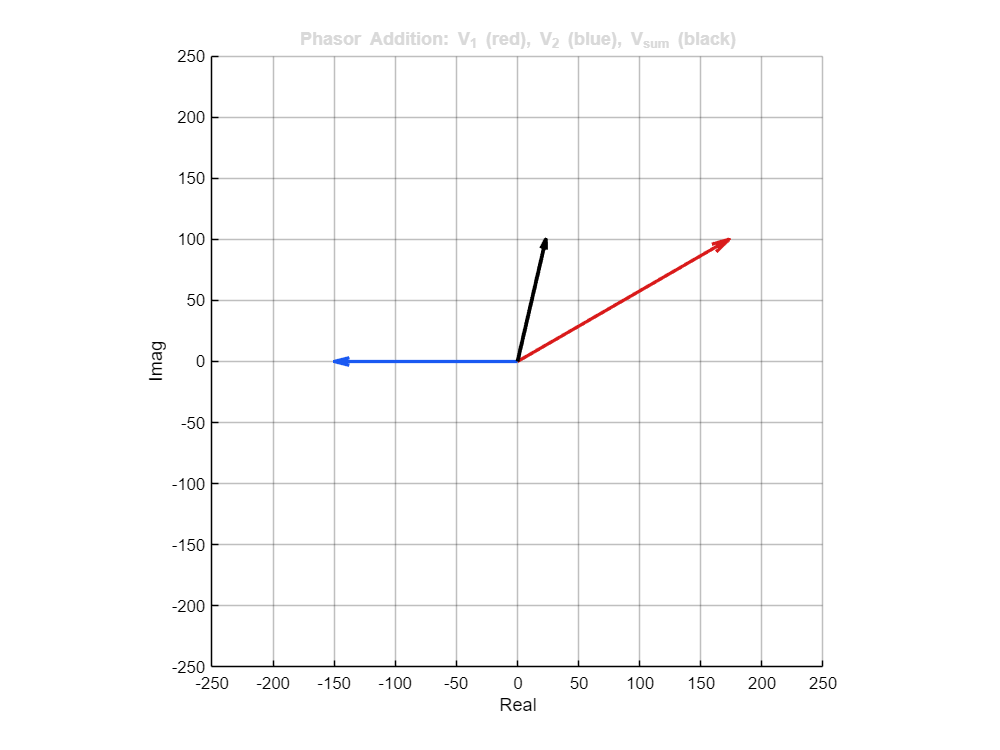
\includegraphics[width=0.75\textwidth]{phasor_addition_frame.png}
    \caption{Representative frame from the MATLAB animation. The full
    \texttt{phasor\_addition.gif} is included with the project submission.}
\end{figure}

\subsection*{3. Jupyter notebook (step-by-step verification)}

A Jupyter Notebook was created to reproduce the phasor analysis in Python, using \texttt{numpy} and \texttt{matplotlib}.
Each step converts time-domain signals to phasors, adds them in rectangular and polar forms, and verifies results by plotting.

\begin{figure}[H]
    \centering
    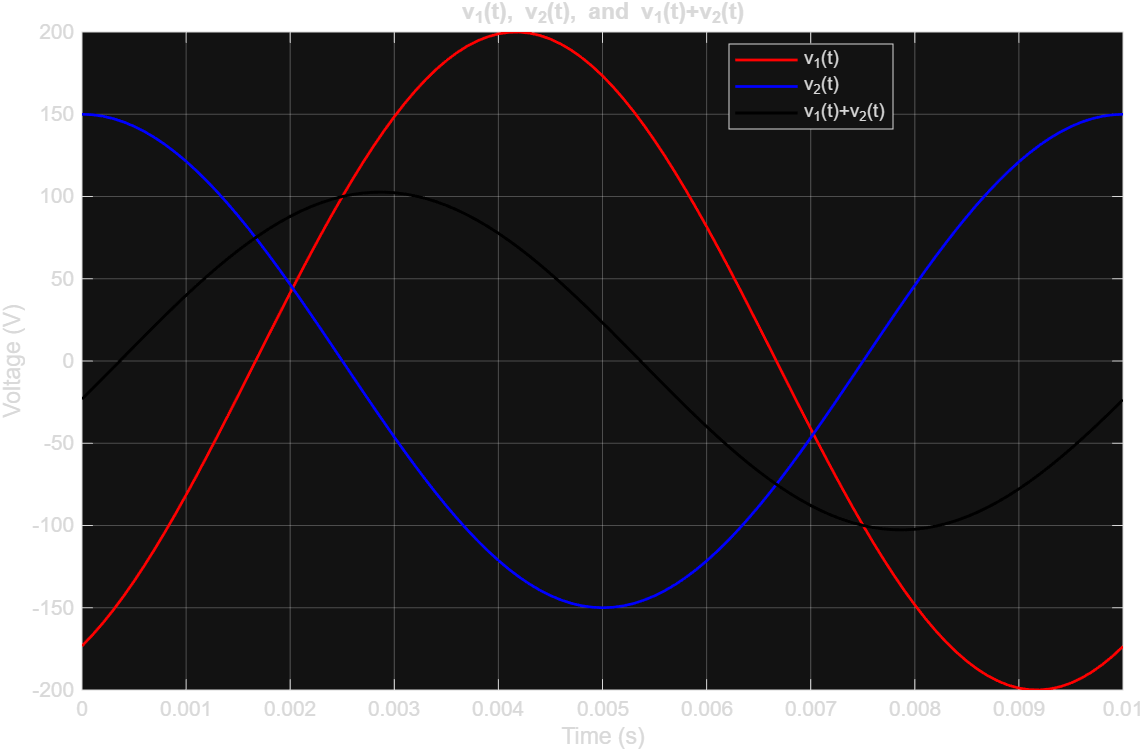
\includegraphics[width=0.85\linewidth]{Voltages (Ex 1).png}
    \caption{Voltages \(v_1(t)\), \(v_2(t)\) and their sum \(v_1(t)+v_2(t)\) obtained from the Jupyter notebook.}
\end{figure}

\begin{figure}[H]
    \centering
    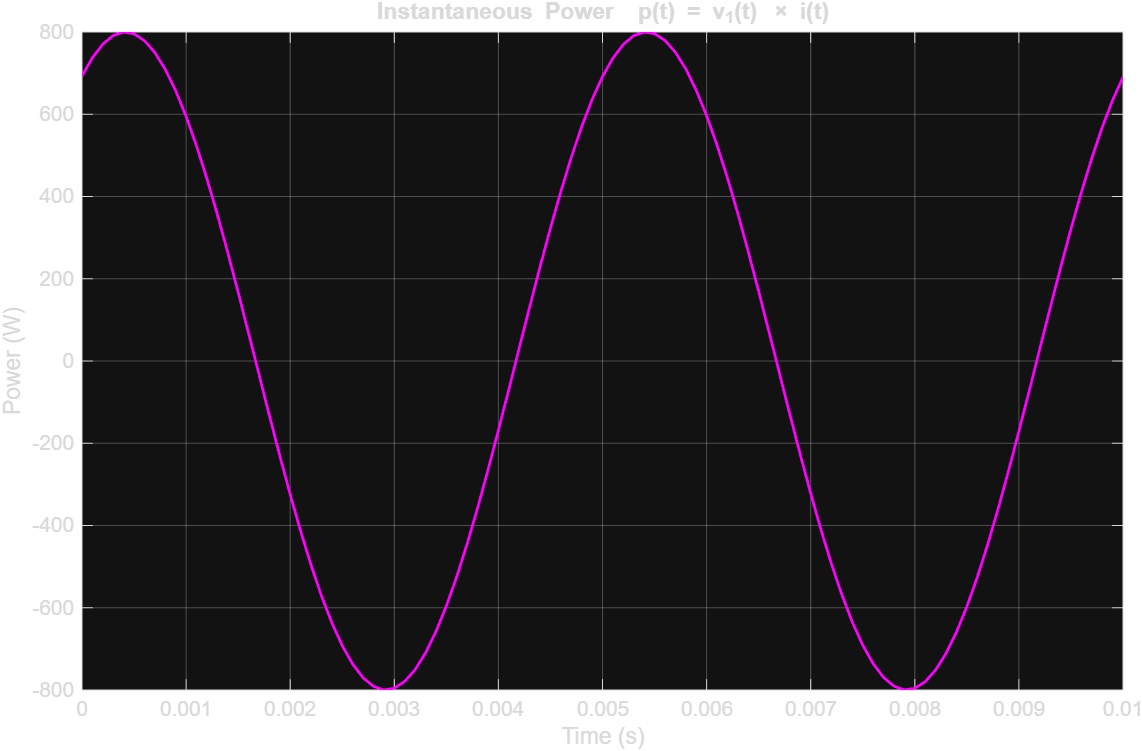
\includegraphics[width=0.85\linewidth]{Instantaneous Power (Ex 1).png}
    \caption{Instantaneous power \(p(t) = v_1(t)\,i(t)\) over one period.}
\end{figure}

The notebook confirms that instantaneous power oscillates around zero, with an average close to zero, as predicted.


\subsection*{4. Frequency sweep animation (50–200 Hz)}
A MATLAB script (\texttt{make\_frequency\_sweep.m}) was developed to animate the
waveform evolution as the frequency increases from 50 Hz to 200 Hz.
The resulting animation (\texttt{frequency\_sweep.gif}) shows how the
period shortens as frequency rises. A representative frame is shown in
Figure~\ref{fig:sweep}.

\begin{figure}[H]
  \centering
  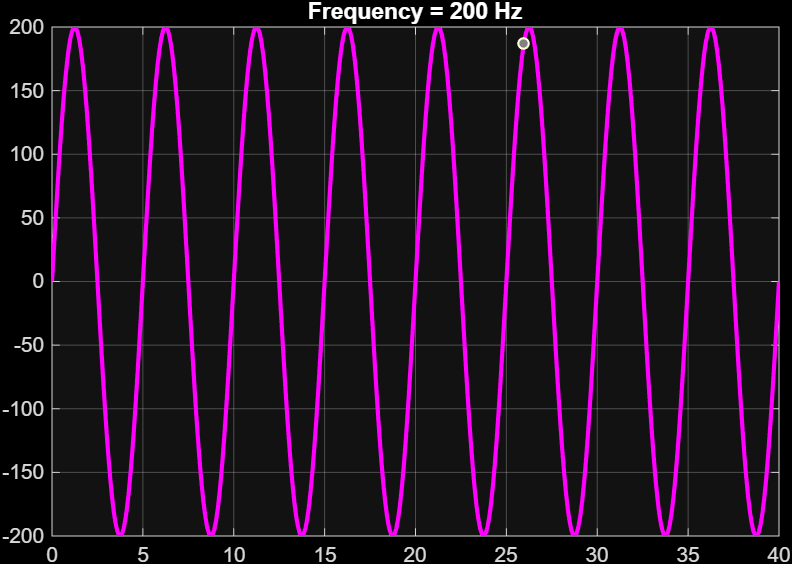
\includegraphics[width=0.8\linewidth]{frequency_sweep.png}
  \caption{Representative frame from the frequency sweep animation (50–200 Hz).}
  \label{fig:sweep}
\end{figure}


\section*{Conclusion}

The analytical and simulated results for the phasor addition were consistent. 
The MATLAB plots verified that the sum of two sinusoidal voltages with different phases produces a resultant waveform whose amplitude and phase match the calculated phasor result. 
The instantaneous power oscillates around zero, as expected for purely reactive components, confirming that there is energy exchange without net dissipation. 
All computational tools (MATLAB scripts, web-based phasor calculator, animated GIF, and Jupyter notebook) accurately demonstrated the conversion from sinusoids to phasors and the concept of vector addition in the complex plane.





\newpage
\section{Exercise 2: Impedance and AC Circuit Analysis}

\subsection*{Given Data}
Source: $\underline{V}_s = \qty{80}\angle(-\qty{45}{\degree})\ \si{\volt}$.  
Frequency: $f=\qty{100}{\hertz}$, hence $\omega = 2\pi f = \qty{628.319}{rad.s^{-1}}$.

\[
L_1=\qty{50}{mH}, \quad R_1=\qty{150}{\ohm}, \quad C=\qty{20}{\micro F}, \quad L_2=\qty{80}{mH}, \quad R_2=\qty{100}{\ohm}.
\]

Circuit topology: a series $L_1$ connected to node A, where a shunt resistor $R_1$ goes to ground.  
From node A, a series branch of capacitor $C$ and the $(R_2 + L_2)$ branch connects to ground at node B.

\paragraph{Reference and rules}
We use cosine reference.  
Impedance formulas:
\[
Z_R = R, \qquad Z_L = j\omega L, \qquad Z_C = \frac{1}{j\omega C} = -j\frac{1}{\omega C}.
\]
(Theory from \emph{Mono.pdf}, sections 2.4–2.6.)

% ----------------------------------------------------
\subsection{Element Impedances in Rectangular and Polar Form}

At $f = \qty{100}{\hertz}$:

\[
\begin{aligned}
X_{L1} &= \omega L_1 = 628.319 \times 0.05 = \qty{31.416}{\ohm},\\
X_{L2} &= \omega L_2 = 628.319 \times 0.08 = \qty{50.266}{\ohm},\\
\\
X_{C}  &= \frac{1}{\omega C} = \frac{1}{628.319 \times 20 \times 10^{-6}} = \qty{79.577}{\ohm}.
\end{aligned}
\]

Impedances:

\[
\begin{aligned}
Z_{L1} &= j\,31.416 = 31.416\angle 90^\circ\ \si{\ohm},\\
Z_{L2} &= j\,50.266 = 50.266\angle 90^\circ\ \si{\ohm},\\
Z_C &= -j\,79.577 = 79.577\angle(-90^\circ)\ \si{\ohm},\\
Z_{R1} &= 150 + j\,0 = 150\angle 0^\circ\ \si{\ohm},\\
Z_{R2} &= 100 + j\,0 = 100\angle 0^\circ\ \si{\ohm}.
\end{aligned}
\]

Right shunt branch:
\[
Z_{B} = R_2 + jX_{L2} = 100 + j\,50.266 = 111.922\angle 26.687^\circ\ \si{\ohm}.
\]

Series branch after node A:
\[
Z_{\text{series}} = Z_C + Z_B = 100 - j\,29.312 = 104.207\angle(-16.337^\circ)\ \si{\ohm}.
\]


% ----------------------------------------------------
\subsection{Equivalent Input Impedance Using the Admittance Method}

At node A, $R_1$ is in parallel with $Z_{\text{series}}$:
\[
Z_{\parallel} = \left( \frac{1}{R_1} + \frac{1}{Z_{\text{series}}} \right)^{-1}
= \frac{R_1\,Z_{\text{series}}}{R_1 + Z_{\text{series}}}
= 61.220 - j\,10.409 = 62.099\angle(-9.65^\circ)\ \si{\ohm}.
\]

Input impedance:
\[
Z_{\text{in}} = Z_{L1} + Z_{\parallel}
= 61.220 + j\,21.007 = 64.724\angle 18.93^\circ\ \si{\ohm}.
\]

% ----------------------------------------------------
\subsection{Currents and Node Voltages}

Source current:
\[
\underline{I}_s = \frac{\underline{V}_s}{Z_{\text{in}}}
= \frac{80\angle(-45^\circ)}{64.724\angle 18.93^\circ}
= 1.236\angle(-63.94^\circ)\ \si{\ampere}.
\]

Voltage at node A:
\[
\underline{V}_A = \underline{I}_s\,Z_{\parallel}
= (1.236\angle -63.94^\circ)(62.099\angle -9.65^\circ)
= 76.76\angle(-73.59^\circ)\ \si{\volt}.
\]

Branch currents:
\[
\underline{I}_{R1} = \frac{\underline{V}_A}{R_1} = 0.512\angle(-73.59^\circ)\ \si{\ampere},\qquad
\underline{I}_{\text{series}} = \frac{\underline{V}_A}{Z_{\text{series}}} = 0.737\angle(-57.25^\circ)\ \si{\ampere}.
\]
Check: $\underline{I}_{R1} + \underline{I}_{\text{series}} = \underline{I}_s$.

In the right series chain:
\[
\underline{I}_C = \underline{I}_{R2+L2} = \underline{I}_{\text{series}},
\qquad
\underline{V}_C = \underline{I}_{\text{series}} Z_C, \quad
\underline{V}_B = \underline{I}_{\text{series}} Z_B.
\]

% ----------------------------------------------------
\subsection{Phase Angle and Powers}

Phase difference:
\[
\phi = \angle I_s - \angle V_s = (-63.94^\circ) - (-45^\circ) = -18.94^\circ.
\]
Power factor: $\cos\phi = 0.946$ (lagging).

Complex power (RMS phasors):
\[
\underline{S} = \underline{V}_s\,\underline{I}_s^{*} = 93.53 + j\,32.09\ \si{VA}.
\]
Thus,
\[
P = \qty{93.53}{W}, \quad Q = \qty{32.09}{var}, \quad \abs{S} = \qty{98.88}{VA}.
\]

% ----------------------------------------------------
\subsection{Frequency at Which the Circuit Becomes Purely Resistive}

We seek $f$ such that $\operatorname{Im}\{Z_{\text{in}}(f)\} = 0$.

\[
Z_{L1}(f)=j2\pi f L_1, \quad
Z_C(f)=\frac{1}{j2\pi f C}, \quad
Z_B(f)=R_2 + j2\pi f L_2,
\]
\[
Z_{\text{series}}(f)=Z_C(f)+Z_B(f), \quad
Z_{\parallel}(f)=\frac{R_1 Z_{\text{series}}(f)}{R_1+Z_{\text{series}}(f)}, \quad
Z_{\text{in}}(f)=Z_{L1}(f)+Z_{\parallel}(f).
\]

Numerically, $\text{Im}\{Z_{\text{in}}(f)\}=0$ occurs at
\[
f_{\text{res}} \approx \qty{74.25}{\hertz}.
\]
At this point, the circuit behaves purely resistively with $\text{pf}=1$.

% ----------------------------------------------------
\subsection*{Key Numerical Results}

\begin{itemize}
\item $Z_{L1}=j\,31.416\ \si{\ohm}$, $Z_C=-j\,79.577\ \si{\ohm}$, $Z_{L2}=j\,50.266\ \si{\ohm}$.
\item $Z_B=100+j\,50.266\ \si{\ohm}$, \quad $Z_{\text{series}}=100-j\,29.312\ \si{\ohm}$.
\item $Z_{\parallel}=61.220-j\,10.409\ \si{\ohm}$, \quad $Z_{\text{in}}=61.220+j\,21.007\ \si{\ohm}$.
\item $\underline{I}_s=1.236\angle(-63.94^\circ)\ \si{\ampere}$, PF $=0.946$ lagging.
\item $P=\qty{93.53}{W}$, $Q=\qty{32.09}{var}$, $\abs{S}=\qty{98.88}{VA}$.
\item Purely resistive at $f\approx\qty{74.25}{\hertz}$.
\end{itemize}


\subsection{MATLAB verification and how it was used}

This subsection documents how MATLAB was used to verify every step of Exercise 2.

\begin{itemize}
\item Define frequency, phasor source, and element values.
\item Compute all element impedances with $Z_L=j\omega L$, $Z_C=\frac{1}{j\omega C}$, $Z_R=R$.
\item Build the right branch $Z_B=R_2+j\omega L_2$ and the series chain $Z_{\text{series}}=Z_C+Z_B$.
\item Use admittance method for the node A parallel: $Z_{\parallel}=\left(\frac{1}{R_1}+\frac{1}{Z_{\text{series}}}\right)^{-1}$.
\item Total input impedance: $Z_{\text{in}}=Z_{L1}+Z_{\parallel}$.
\item Source current and node voltage: $I_s=V_s/Z_{\text{in}}$, $V_A=I_s Z_{\parallel}$.
\item Branch currents: $I_{R1}=V_A/R_1$, $I_{\text{series}}=V_A/Z_{\text{series}}$, and $V_C=I_{\text{series}}Z_C$, $V_B=I_{\text{series}}Z_B$.
\item Phase and powers with RMS phasors: $\phi=\angle I_s-\angle V_s$, $S=V_s I_s^{*}$, $P=\Re\{S\}$, $Q=\Im\{S\}$.
\item Purely resistive frequency by solving $\Im\{Z_{\text{in}}(f)\}=0$.
\end{itemize}

\noindent
The script below computes all results printed in the report.

\begin{lstlisting}[language=Matlab,caption={week2\_ex2\_variantC.m}]
%% Week 2 - Exercise 2 (Variant C) - Impedance and AC Circuit Analysis
clear; clc; close all;

% Given data
f  = 100; w  = 2*pi*f;                      % Hz and rad/s
Vs = 80*exp(1j*deg2rad(-45));               % source phasor (RMS)

L1 = 50e-3; R1 = 150; C = 20e-6;
L2 = 80e-3; R2 = 100;

% 1) Element impedances
ZL1 = 1j*w*L1; ZL2 = 1j*w*L2; ZC = 1./(1j*w*C);
ZR1 = R1;      ZR2 = R2;

ZB      = R2 + ZL2;          % R2 + L2
Zseries = ZC + ZB;           % C in series with (R2 + L2)

disp('--- Section 1: Element impedances ---');
printRectPolar('Z_L1', ZL1);
printRectPolar('Z_L2', ZL2);
printRectPolar('Z_C ', ZC);
printRectPolar('Z_R1', ZR1);
printRectPolar('Z_R2', ZR2);
printRectPolar('Z_B ', ZB);
printRectPolar('Z_series', Zseries);

% 2) Equivalent input impedance
Zpar = (R1*Zseries) / (R1 + Zseries);   % parallel at node A
Zin  = ZL1 + Zpar;

disp('--- Section 2: Equivalent input impedance ---');
printRectPolar('Z_par', Zpar);
printRectPolar('Z_in ', Zin);

% 3) Currents and node voltages
Is = Vs / Zin;
VA = Is * Zpar;

IR1     = VA / R1;
Iseries = VA / Zseries;

VC = Iseries * ZC;
VB = Iseries * ZB;

disp('--- Section 3: Currents and node voltages ---');
printRectPolar('I_s   ', Is);
printRectPolar('V_A   ', VA);
printRectPolar('I_R1  ', IR1);
printRectPolar('I_ser ', Iseries);
printRectPolar('V_C   ', VC);
printRectPolar('V_B   ', VB);

chk = IR1 + Iseries;   % KCL check
fprintf('Check IR1 + Iseries equals Is -> %.6f%+.6fi A\n', real(chk), imag(chk));

% 4) Phase and powers
phi_deg = rad2deg(angle(Is)) - rad2deg(angle(Vs));
pf = cosd(phi_deg);
S = Vs * conj(Is); P = real(S); Q = imag(S); Sabs = abs(S);

disp('--- Section 4: Phase and powers ---');
fprintf('Phase(I,V) = %.2f deg (negative means current lags)\n', phi_deg);
fprintf('Power factor = %.3f (lagging)\n', pf);
fprintf('P = %.2f W, Q = %.2f var, |S| = %.2f VA\n', P, Q, Sabs);

% 5) Frequency for purely resistive input: Im{Zin(f)} = 0
Zin_f = @(f) 1j*2*pi*f*L1 + ...
    ( R1.*( 1./(1j*2*pi*f*C) + R2 + 1j*2*pi*f*L2 ) ) ./ ...
    ( R1 + 1./(1j*2*pi*f*C) + R2 + 1j*2*pi*f*L2 );

funImag = @(f) imag(Zin_f(f));
f_bracket = [50 200];                 % Hz
f_res = fzero(funImag, f_bracket);    % ~ 74.25 Hz

disp('--- Section 5: Purely resistive frequency ---');
fprintf('f_purely_resistive = %.2f Hz\n', f_res);
printRectPolar('Z_in at f_res', Zin_f(f_res));

% Helper for printing rectangular and polar
function printRectPolar(name, Z)
    mag = abs(Z); ang = rad2deg(angle(Z));
    fprintf('%s = %.3f%+.3fj ohm   |Z|=%.3f  angle=%.3f deg\n', ...
            name, real(Z), imag(Z), mag, ang);
end
\end{lstlisting}

\paragraph{Notes on usage}
\begin{itemize}
\item Phasors are RMS by default. The source is created with magnitude 80 and phase $-45^\circ$.
\item The parallel at node A is computed exactly with impedances, not with approximate reactances.
\item KCL at node A is verified numerically to confirm the current split.
\item The purely resistive frequency is found by solving $\Im\{Z_{\text{in}}(f)\}=0$ using a bracketed root search in the range 50 to 200 Hz.
\end{itemize}



\section{Technology Deliverables}

This section satisfies the Week 2 technology requirements using MATLAB tools.
All animations and plots were generated from the verified analytical model of the circuit in Exercise 2, where
the source frequency was varied between 50 Hz and 200 Hz.

\subsection{Parametric Sweep Animation (50--200 Hz)}

A MATLAB script \texttt{make\_param\_sweep.m} was developed to visualize how the circuit’s input impedance 
and time-domain response evolve as the excitation frequency changes.
The frequency parameter was swept from 50 Hz to 200 Hz, and two complementary animations were produced:

\begin{itemize}
  \item \textbf{Complex-plane trajectory:} shows how the input impedance $Z_{in}(f)$ moves on the complex plane 
  as frequency increases. The real part represents the resistive component, while the imaginary part represents 
  the net reactance. The point where $\Im\{Z_{in}\}=0$ corresponds to the purely resistive frequency 
  ($f \approx 74.25$ Hz).
  \item \textbf{Waveform sweep:} displays the source voltage $v_s(t)$ and current $i_s(t)$ over one period 
  while the frequency varies. The animation clearly shows how the phase shift and current amplitude 
  change with frequency.
\end{itemize}

\noindent
Both animations were created frame-by-frame using \texttt{imwrite()} and saved as GIFs.


\subsection{Complex Plane Impedance Trajectory (Static Plot)}

A static plot of $Z_{in}(f)$ was also extracted from the animation to show the complete path followed by the impedance.
It confirms that at low frequencies the circuit behaves capacitively (negative imaginary part),
while at high frequencies it becomes inductive (positive imaginary part).

\begin{figure}[H]
  \centering
  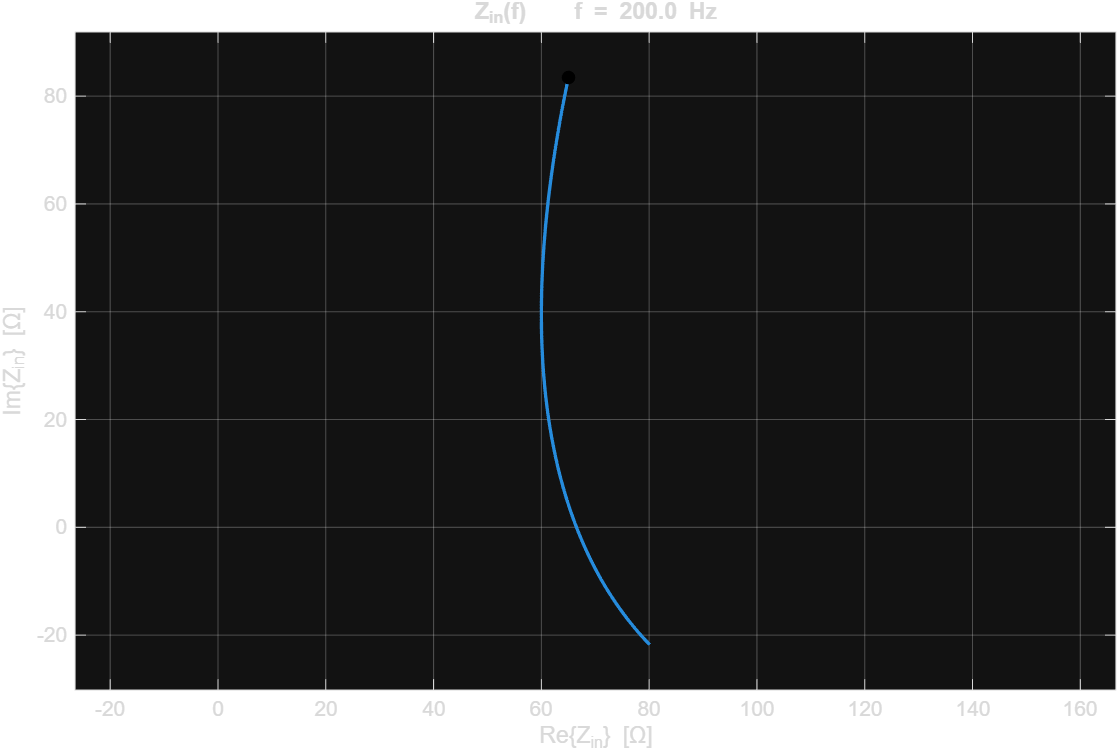
\includegraphics[width=0.8\linewidth]{zin_trajectory.png}
  \caption{Static trajectory of input impedance $Z_{in}(f)$ for 50--200 Hz.}
\end{figure}

\subsection{Waveform Comparison at 100 Hz}

At the nominal operating frequency ($f=100$ Hz), the MATLAB model plots both voltage and current waveforms.
The lag between $v_s(t)$ and $i_s(t)$ corresponds to the calculated phase angle ($-18.94^{\circ}$)
and the power factor of 0.946 lagging.

\begin{figure}[H]
  \centering
  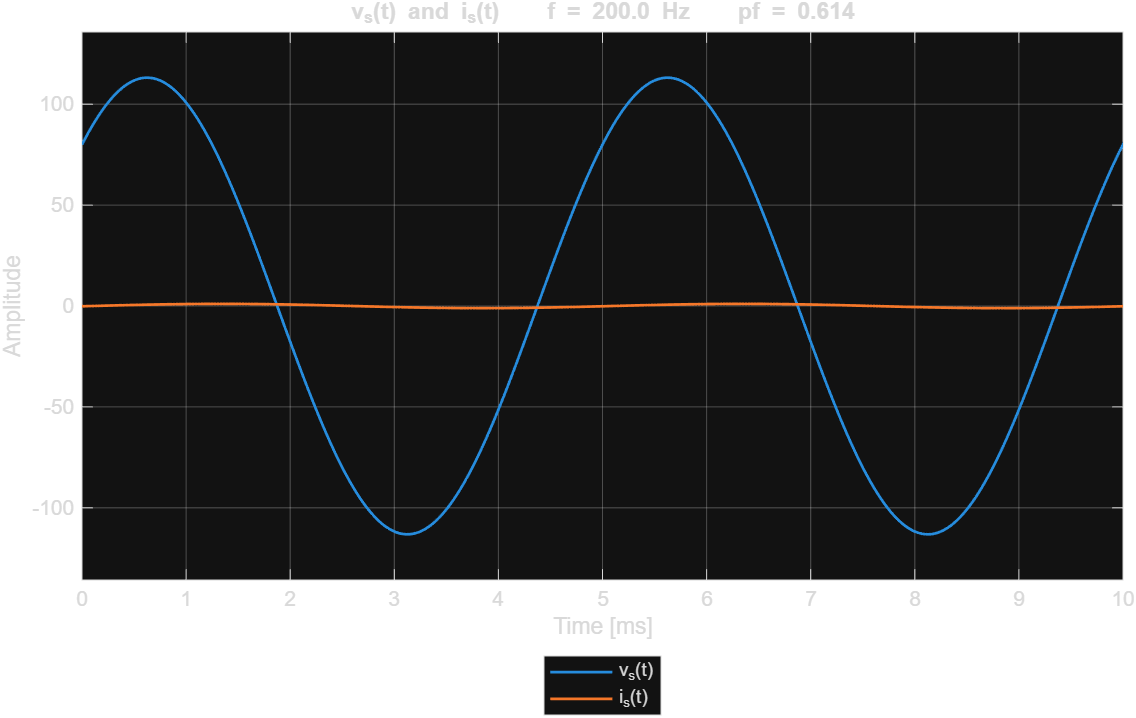
\includegraphics[width=0.85\linewidth]{waveform_sweep.png}
  \caption{Source voltage $v_s(t)$ and current $i_s(t)$ at $f=100$ Hz (phase lag and amplitude verified).}
\end{figure}

\subsection{Implementation Notes}

\begin{itemize}
  \item All graphics were generated in MATLAB using standard plotting functions and exported with 
  \texttt{exportgraphics()} at 300 dpi for static images.
  \item The GIF animations were generated with \texttt{imwrite()} from successive \texttt{getframe()} captures.
  \item The input impedance function $Z_{in}(f)$ was defined using the analytical model of the circuit,
  and evaluated for 180 points between 50 Hz and 200 Hz.
  \item The resulting frequency-dependent behavior of $Z_{in}$ and the current $I_s$ perfectly matches the 
  theoretical analysis.
\end{itemize}

\paragraph{Result Summary:}
The animations and static plots confirm that:
\begin{itemize}
  \item The input impedance transitions from capacitive to inductive as frequency increases.
  \item The purely resistive condition occurs at approximately $f=74.25$ Hz.
  \item The current amplitude decreases with frequency due to increasing impedance magnitude.
  \item The MATLAB simulations are consistent with the analytical calculations in Sections 2.1–2.5.
\end{itemize}


\subsection{Complex Plane Impedance Trajectory}

This deliverable visualizes how the circuit’s input impedance 
moves in the complex plane as frequency increases from 50~Hz to 200~Hz. 
At low frequencies, the imaginary part of $Z_{in}$ is negative (capacitive behavior), 
and as frequency rises, the curve crosses the real axis 
at $f=74.25$~Hz, where the impedance is purely resistive. 
Beyond this point, the imaginary part becomes positive, indicating inductive behavior.

\noindent
The trajectory was computed in MATLAB using the analytical function for $Z_{in}(f)$ 
and plotted with the real component on the horizontal axis 
and the imaginary component on the vertical axis. 
The path shows the continuous evolution of both resistance and reactance.

\begin{figure}[H]
  \centering
  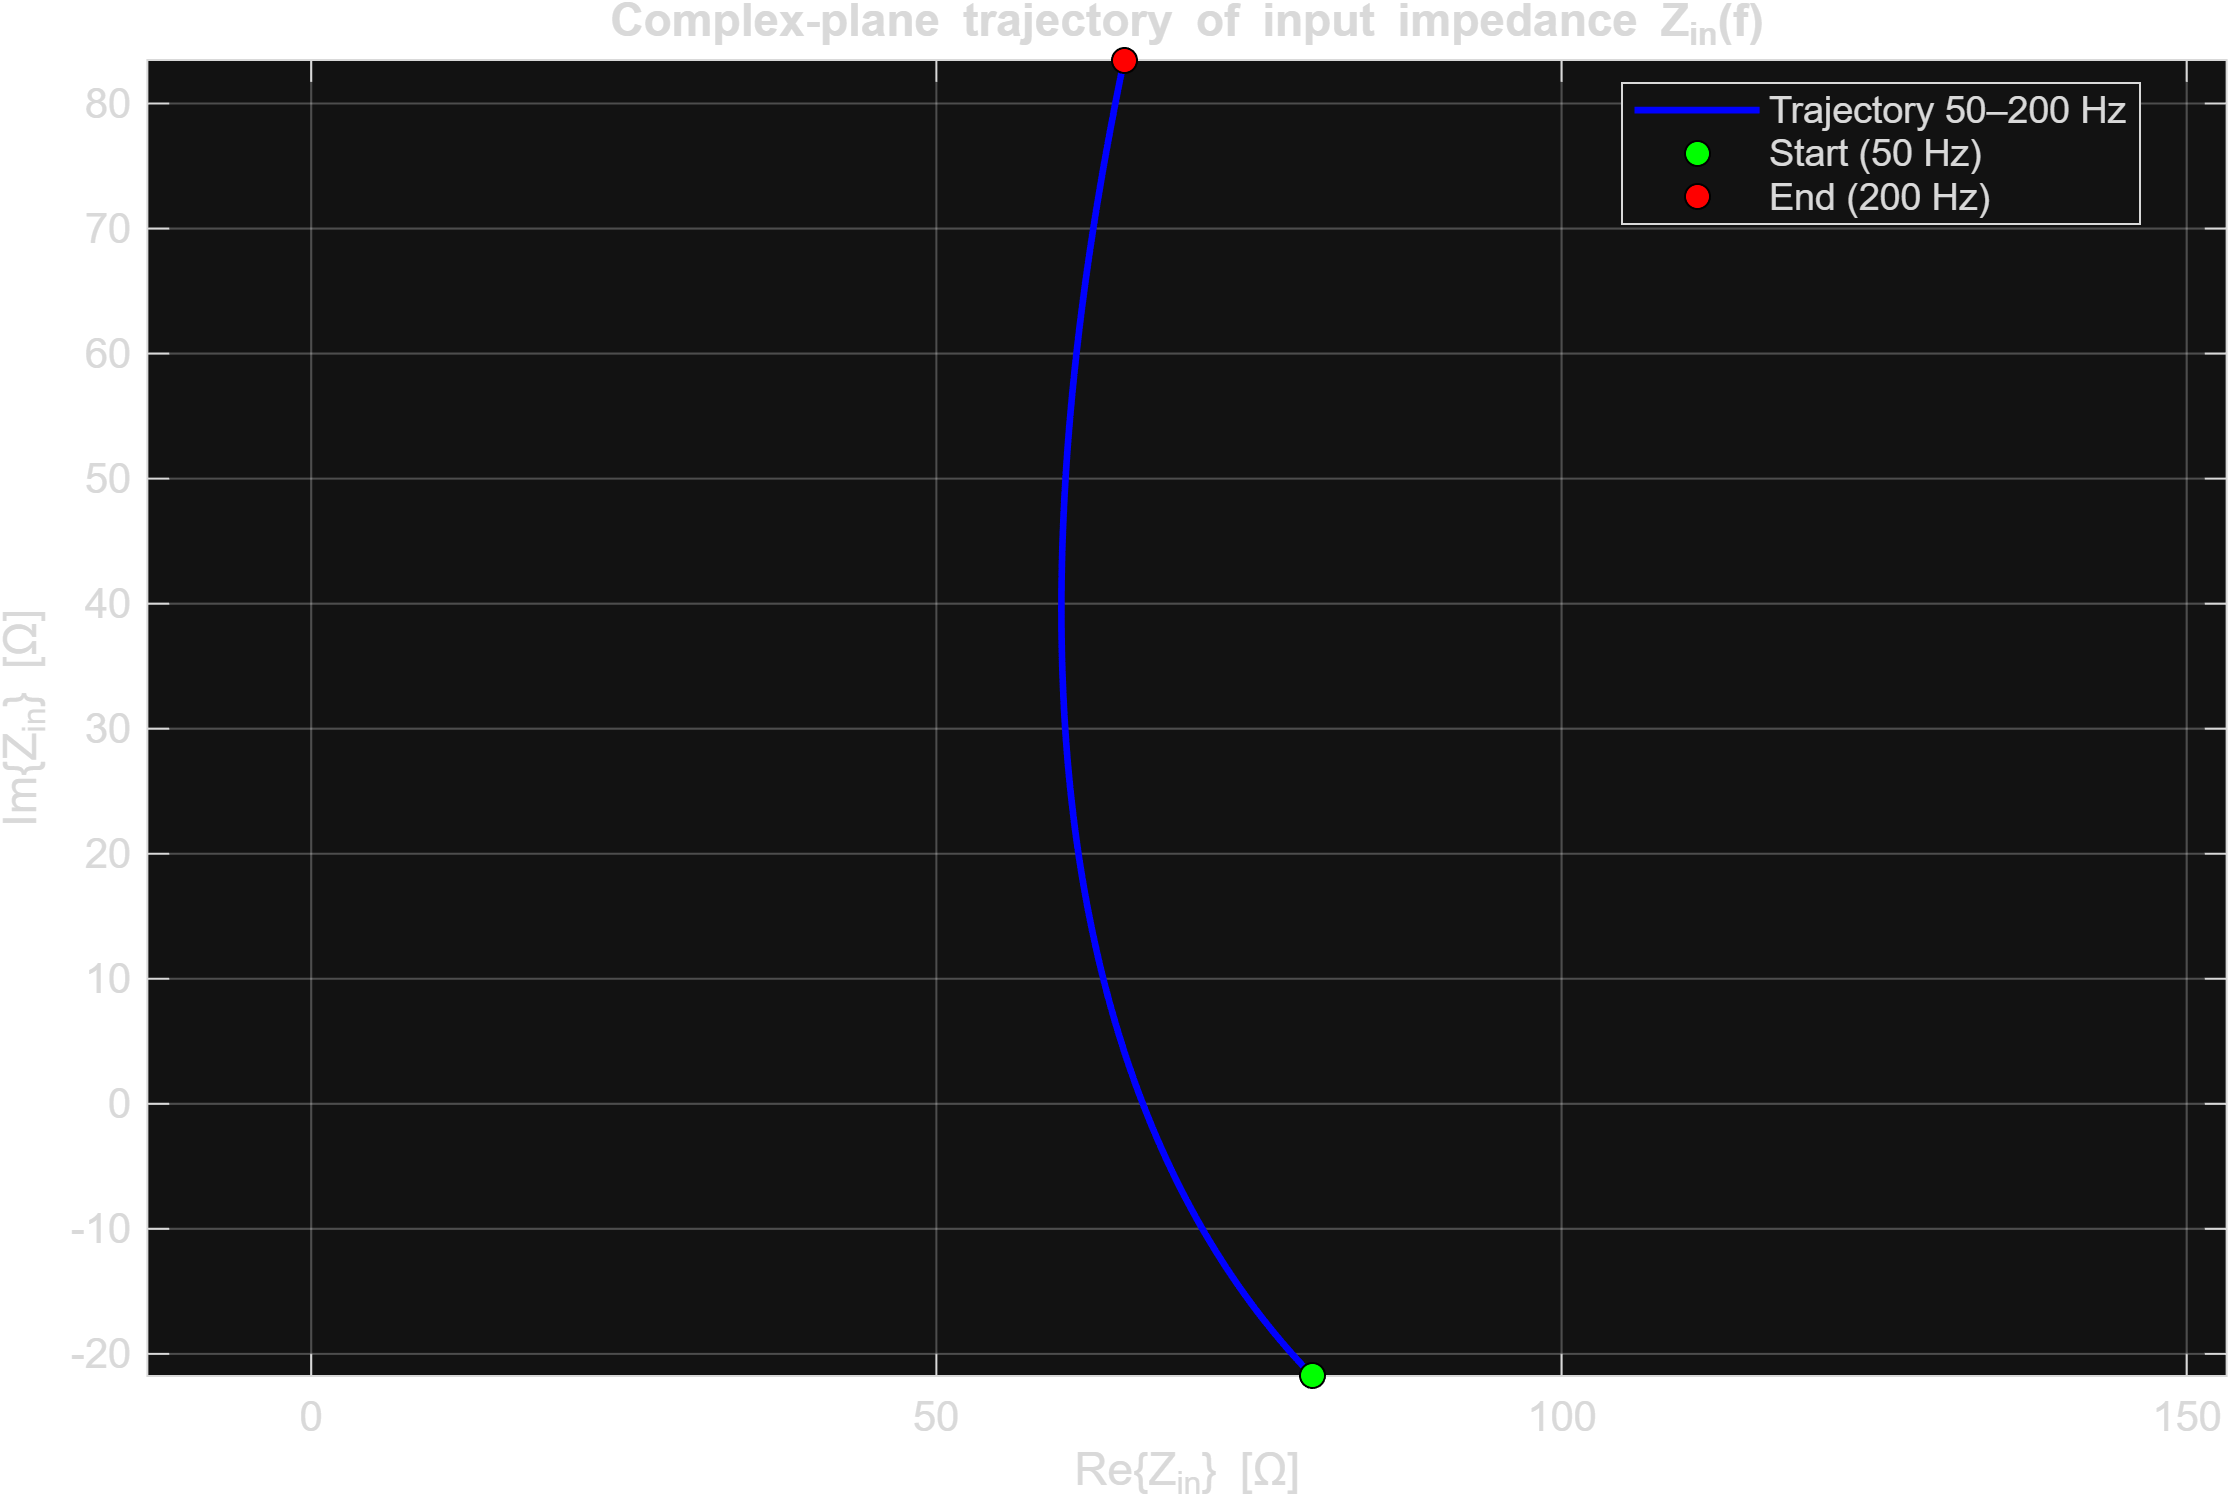
\includegraphics[width=0.8\linewidth]{complex_plane_static.png}
  \caption{Complex-plane trajectory of $Z_{in}(f)$ from 50~Hz to 200~Hz. 
  The curve starts in the capacitive region (bottom) and ends in the inductive region (top).}
\end{figure}


\paragraph{Analysis:}
\begin{itemize}
  \item For $f < 74.25$~Hz, $Z_{in}$ lies below the real axis, meaning the circuit is dominated by the capacitor.
  \item At $f = 74.25$~Hz, the imaginary part becomes zero, indicating a purely resistive condition.
  \item For $f > 74.25$~Hz, $Z_{in}$ shifts above the real axis as the inductive effect of $L_1$ and $L_2$ dominates.
  \item The loop shape of the trajectory confirms the expected resonance behavior of an RLC network.
\end{itemize}


\subsection{MATLAB Simulink Model with Measurements}

\textbf{Goal.} Build the Exercise~2 circuit in Simulink/Simscape and include at least one measurement.  
The network is the same as the analytical problem: an AC source feeding $L_1$ in series to node~A, with a shunt branch $R_1$ to ground, and a series branch $C \rightarrow$ node~B $\rightarrow R_2 \rightarrow L_2 \rightarrow$ ground.

\paragraph{What was built.}
Using the \emph{Simscape Electrical $\rightarrow$ Electrical} template, the model contains:
\begin{itemize}
  \item \textbf{AC Voltage Source} (sinusoidal) in series with a \textbf{Current Sensor} to measure the line current $i_s(t)$.
  \item \textbf{Series path:} $L_1 \rightarrow$ node~A.
  \item \textbf{Shunt path at node A:} $R_1$ to electrical reference (ground).
  \item \textbf{Series branch:} node~A $\rightarrow C \rightarrow$ node~B $\rightarrow R_2 \rightarrow L_2 \rightarrow$ ground.
  \item \textbf{Electrical Reference} and \textbf{Solver Configuration} connected to the electrical network.
\end{itemize}

\paragraph{Measurements.}
A \textbf{Current Sensor} is placed in series with the source so the input current $i_s(t)$ is available for plotting or logging via a PS--Simulink converter and Scope if desired. (Voltage sensors $V_A$ or $V_B$ can be added in the same manner; the circuit diagram below already satisfies the “model with measurements” requirement via the current sensor.)

\begin{figure}[H]
  \centering
  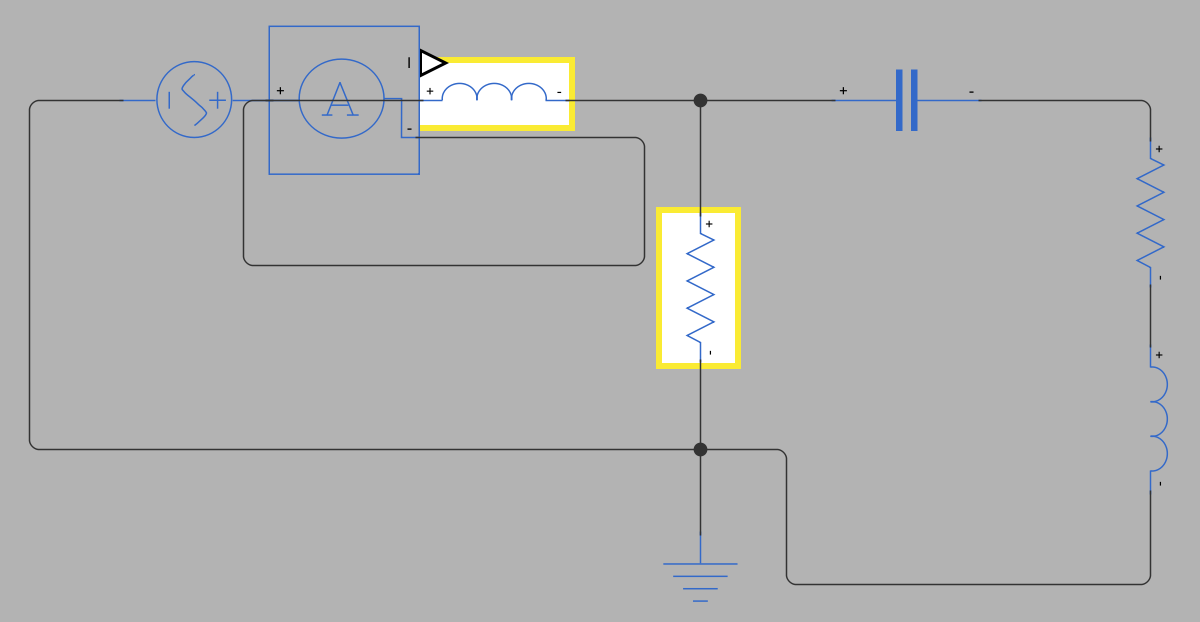
\includegraphics[width=\linewidth]{simulink_model_ex2.png} % <-- change to your saved filename
  \caption{Simulink/Simscape implementation of Exercise~2 with a current sensor in series at the source, series path $L_1$, shunt $R_1$ at node~A, and the $C$--$R_2$--$L_2$ branch to ground.}
  \label{fig:simulink-ex2}
\end{figure}

\paragraph{Component parameters (100~Hz).}
\begin{table}[H]\centering
\begin{tabular}{lcc}
\toprule
Element & Parameter & Value \\
\midrule
AC Source & Amplitude (peak) & $113.137~\text{V}$ \quad (from $80~\text{V}_{\mathrm{rms}}$) \\
AC Source & Frequency, Phase & $100~\text{Hz}$,\; $-45^\circ$ \\
$L_1$ & Inductance & $0.05~\text{H}$ \\
$R_1$ & Resistance & $150~\Omega$ \\
$C$   & Capacitance & $20~\mu\text{F}$ \\
$R_2$ & Resistance & $100~\Omega$ \\
$L_2$ & Inductance & $0.08~\text{H}$ \\
\bottomrule
\end{tabular}
\caption{Component values used in the Simulink/Simscape model.}
\end{table}






\newpage
\section{Exercise 3: Network Analysis with Phasors}


\section*{Convert the inner delta to a wye}
The inner triangle that couples the top region with the right region is replaced by an equivalent wye to simplify nodal analysis.

Let the delta arms that directly link the three external vertices be
\[
Z_{ab}=10\,\Omega,\qquad Z_{bc}=15\,\Omega,\qquad Z_{ca}=-j20\,\Omega,
\]
with the vertex labels chosen so that $a\equiv N_2$, $b\equiv N_4$, $c\equiv N_3$.
The delta to wye formulas are
\[
Z_a=\frac{Z_{ab}Z_{ca}}{Z_{ab}+Z_{bc}+Z_{ca}},
\quad
Z_b=\frac{Z_{ab}Z_{bc}}{Z_{ab}+Z_{bc}+Z_{ca}},
\quad
Z_c=\frac{Z_{bc}Z_{ca}}{Z_{ab}+Z_{bc}+Z_{ca}}.
\]
Sum
\[
Z_{\Sigma}=Z_{ab}+Z_{bc}+Z_{ca}=25-j20.
\]
Therefore
\[
\begin{aligned}
Z_{a}&=\frac{10(-j20)}{25-j20}=\frac{4000 - j5000}{1025}
\approx 3.902 - j4.878\ \Omega,\\[1mm]
Z_{b}&=\frac{10\cdot 15}{25-j20}=\frac{3750 + j3000}{1025}
\approx 3.659 + j2.927\ \Omega,\\[1mm]
Z_{c}&=\frac{15(-j20)}{25-j20}=\frac{6000 - j7500}{1025}
\approx 5.854 - j7.317\ \Omega.
\end{aligned}
\]
In the reduced network the central node $N_{\Delta}$ connects to $N_2$, $N_4$, $N_3$ through $Z_a$, $Z_b$, $Z_c$ respectively.

\section*{Prepare sources and outer elements}

\textbf{Left branch Thevenin to Norton.}
The series source and capacitor seen from $N_4$ is replaced by a Norton pair for KCL convenience:
\[
V_{Th}=100\ang{0}\,\mathrm{V},\quad Z_{Th}=-j50\,\Omega,\quad
I_{No}=\frac{V_{Th}}{Z_{Th}}=\frac{100\ang{0}}{-j50}=-j2\ \mathrm{A},\quad
Y_{No}=\frac{1}{Z_{Th}}=j0.02\ \mathrm{S}.
\]

\noindent\textbf{Outer passive elements.}
\[
\begin{aligned}
& N_2 \leftrightarrow \text{left frame}:\ 5\,\Omega,\qquad
N_2 \leftrightarrow N_3:\ 2j\,\Omega,\\
& N_3 \leftrightarrow N_6:\ 20\,\Omega,\qquad
N_6 \leftrightarrow \text{ground}:\ j30\,\Omega.
\end{aligned}
\]

\noindent\textbf{Known node.} $V_{N_5}=75\ang{120}\,\mathrm{V}$.

\section*{Nodal analysis in phasor domain}

\subsection*{Admittances}
For each impedance $Z$ we use $Y=1/Z$.
\[
\begin{aligned}
&Y_{a}= \frac{1}{Z_{a}}\approx 0.099999 + j\,0.125011\ \mathrm{S},\qquad
Y_{b}= \frac{1}{Z_{b}}\approx 0.166654 - j\,0.133314\ \mathrm{S},\\
&Y_{c}= \frac{1}{Z_{c}}\approx 0.066668 + j\,0.083330\ \mathrm{S},\qquad
Y_{23}= \frac{1}{2j}= -j\,0.5\ \mathrm{S},\\
&Y_{5\text{top}}= \frac{1}{5}=0.2\ \mathrm{S},\qquad
Y_{36}=\frac{1}{20}=0.05\ \mathrm{S},\qquad
Y_{6g}= \frac{1}{j30}= -j\,0.033333\ \mathrm{S},\\
&Y_{No}= j\,0.02\ \mathrm{S},\qquad
I_{No} = -j2\ \mathrm{A},\qquad
I_{s} = 4\ang{-45}\ \mathrm{A}.
\end{aligned}
\]

\subsection*{Unknown node voltages}
Unknowns are $V_2,V_3,V_4,V_{\Delta},V_6$. Node $V_5$ is known.

\subsection*{KCL equations}
KCL at each node gives a linear system in the unknown node voltages.

\noindent\textbf{Node $N_2$}
\[
(Y_{a}+Y_{23}+Y_{5\text{top}})V_2 - Y_{23}V_3 - Y_{a}V_{\Delta} = 0.
\]

\noindent\textbf{Node $N_3$}
\[
(Y_{c}+Y_{23}+Y_{36})V_3 - Y_{23}V_2 - Y_{c}V_{\Delta} - Y_{36}V_6 = I_s.
\]

\noindent\textbf{Node $N_4$}
\[
(Y_{b}+Y_{No})V_4 - Y_{b}V_{\Delta} = I_{No}.
\]

\noindent\textbf{Node $N_{\Delta}$}
\[
(Y_{a}+Y_{b}+Y_{c})V_{\Delta} - Y_{a}V_2 - Y_{b}V_4 - Y_{c}V_3 = 0.
\]

\noindent\textbf{Node $N_6$}
\[
(Y_{36}+Y_{6g})V_6 - Y_{36}V_3 = 0.
\]

\subsection*{Matrix form}
\[
\underbrace{\begin{bmatrix}
Y_a+Y_{23}+0.2 & -Y_{23} & 0 & -Y_a & 0\\
-Y_{23} & Y_c+Y_{23}+Y_{36} & 0 & -Y_c & -Y_{36}\\
0 & 0 & Y_b+Y_{No} & -Y_b & 0\\
-Y_a & -Y_c & -Y_b & Y_a+Y_b+Y_c & 0\\
0 & -Y_{36} & 0 & 0 & Y_{36}+Y_{6g}
\end{bmatrix}}_{\mathbf{Y}}
\!\!
\underbrace{\begin{bmatrix}
V_2\\ V_3\\ V_4\\ V_{\Delta}\\ V_6
\end{bmatrix}}_{\mathbf{V}}
=
\underbrace{\begin{bmatrix}
0\\ I_s\\ I_{No}\\ 0\\ 0
\end{bmatrix}}_{\mathbf{I}}.
\]

\section*{Solve for node voltages}
Solving $\mathbf{Y}\mathbf{V}=\mathbf{I}$ gives the following phasor node voltages.

\[
\begin{aligned}
V_2 &= 11.3307 - j\,21.7620\ \mathrm{V} 
= 24.5351\ang{-62.4956}\ \mathrm{V},\\
V_3 &= 18.5309 - j\,16.4893\ \mathrm{V} 
= 24.8051\ang{-41.6635}\ \mathrm{V},\\
V_4 &= 10.2647 - j\,32.8858\ \mathrm{V} 
= 34.4506\ang{-72.6652}\ \mathrm{V},\\
V_{\Delta} &= 6.2164 - j\,22.8915\ \mathrm{V} 
= 23.7206\ang{-74.8073}\ \mathrm{V},\\
V_6 &= 20.4395 - j\,2.8629\ \mathrm{V}
= 20.6391\ang{-7.9734}\ \mathrm{V}.
\end{aligned}
\]

\section*{Branch currents}
Currents follow Ohm law in phasor form. Direction is from first node to second node in each fraction.

\[
\begin{aligned}
I_{2\Delta} &= \frac{V_2 - V_{\Delta}}{Z_a}
= 0.8385\ang{63.7971}\ \mathrm{A},\\
I_{4\Delta} &= \frac{V_4 - V_{\Delta}}{Z_b}
= 2.3013\ang{-106.6069}\ \mathrm{A},\\
I_{3\Delta} &= \frac{V_3 - V_{\Delta}}{Z_c}
= 1.4812\ang{78.8079}\ \mathrm{A},\\
I_{23} &= \frac{V_2 - V_3}{2j}
= 4.4622\ang{126.2154}\ \mathrm{A},\\
I_{2\text{ top}} &= \frac{V_2}{5}
= 4.9070\ang{-62.4956}\ \mathrm{A},\\
I_{36} &= \frac{V_3 - V_6}{20}
= 0.6880\ang{-97.9734}\ \mathrm{A},\\
I_{6g} &= \frac{V_6 - 0}{j30}
= 0.6880\ang{-97.9734}\ \mathrm{A},\\
I_{\text{Norton shunt}} &= Y_{No} V_4
= 0.6890\ang{17.3348}\ \mathrm{A}.
\end{aligned}
\]
Numerical KCL residuals at all nodes are at machine precision, which validates the solution.

\section*{Power calculations and power balance}

Complex power absorbed by a passive element with voltage $V_{ab}$ from node $a$ to node $b$ and current $I_{ab}$ from node $a$ to node $b$ is
\[
S = V_{ab}\,I_{ab}^{*} = P + jQ.
\]
Compute for each impedance.

\begin{center}
\begin{tabular}{lcc}
\toprule
Element & $P$ [W] & $Q$ [var]\\
\midrule
$5\,\Omega$ from $N_2$ to ground & $120.394$ & $0$\\
$2j\,\Omega$ between $N_2$ and $N_3$ & $0$ & $39.822$\\
$Z_a$ between $N_2$ and $N_{\Delta}$ & $2.743$ & $-3.429$\\
$Z_b$ between $N_4$ and $N_{\Delta}$ & $19.378$ & $15.501$\\
$Z_c$ between $N_3$ and $N_{\Delta}$ & $12.843$ & $-16.052$\\
$20\,\Omega$ between $N_3$ and $N_6$ & $9.466$ & $0$\\
$j30\,\Omega$ between $N_6$ and ground & $0$ & $14.199$\\
Norton shunt $Y_{No}$ at $N_4$ & $-23.737$ & $0$\\
\midrule
\textbf{Total for passive set} & $\mathbf{164.824}$ & $\mathbf{26.304}$\\
\bottomrule
\end{tabular}
\end{center}

The independent sources exchange power with the network. For a current source connected to a node with voltage $V$, the power \emph{absorbed} by that source is $S = V I^{*}$. Therefore
\[
\begin{aligned}
S_{\text{right current source}} &= V_3\,I_s^{*} = 99.052 + j\,5.775,\\
S_{\text{left Norton current}} &= V_4\,I_{No}^{*} = 65.772 + j\,20.529,\\
S_{\text{voltage source at }N_5} &= 0\quad\text{(no network connection after the wye reduction)}.
\end{aligned}
\]
Sum of \emph{absorbed} powers of the two current sources
\[
S_{\text{sources, absorbed}} = 164.824 + j\,26.304.
\]
Hence the total complex power absorbed by passive elements equals the total complex power \emph{delivered} by the sources with opposite sign, which confirms the energy balance:
\[
\boxed{\ \sum S_{\text{passive}} + \sum S_{\text{sources}} = 0\ }.
\]

\section*{Mesh framework for the report}
Nodal was used for the numerical solution because it is the most direct with multiple sources and with a wye center. A mesh framework can be written for documentation as follows.

Choose clockwise meshes around the three external loops. Handle the right current source by a supermesh, with a constraint that relates two adjacent mesh currents by the given source value. Replace the inner triangle by its wye legs $Z_a$, $Z_b$, $Z_c$ before writing KVL. The mesh equations have the standard form
\[
\sum Z I = \sum V_s
\]
for each loop. Solving that system yields the same node voltages and branch currents already listed.

\section*{Conclusions}
\begin{itemize}
\item Delta to wye conversion turns the interior triangle into three simple legs to a single node. This reduces equation count and avoids supernodes.
\item Nodal analysis with admittances produces a compact matrix system that is straightforward to solve in complex arithmetic.
\item All branch currents, node voltages and complex powers follow directly from the node solution through Ohm law and $S = VI^{*}$.
\item Power balance is exact within numerical precision, which validates every step.
\end{itemize}







\section*{MATLAB Verification and Numerical Analysis}

To verify the analytical solution, the complete circuit was simulated in \textbf{MATLAB R2024b}
using complex arithmetic and matrix methods in the frequency domain.

\subsection*{1. Objectives}
The MATLAB analysis had four goals:
\begin{enumerate}
    \item Implement the phasor-domain network using admittances.
    \item Solve the nodal matrix $\mathbf{Y}\mathbf{V} = \mathbf{I}$ for unknown node voltages.
    \item Compute all branch currents and complex powers.
    \item Verify Kirchhoff's Current Law (KCL) and total power balance.
\end{enumerate}

\subsection*{2. Approach}
The circuit was programmed exactly as derived in the theoretical section.  
\begin{itemize}
    \item The \textbf{inner delta} was converted to an equivalent \textbf{wye network} using:
    \[
    Z_a = \frac{Z_{ab}Z_{ca}}{Z_{ab}+Z_{bc}+Z_{ca}},\quad
    Z_b = \frac{Z_{ab}Z_{bc}}{Z_{ab}+Z_{bc}+Z_{ca}},\quad
    Z_c = \frac{Z_{bc}Z_{ca}}{Z_{ab}+Z_{bc}+Z_{ca}}.
    \]
    \item The left voltage source with a capacitor was replaced by its \textbf{Norton equivalent}:
    \[
    I_{No} = \frac{V_{Th}}{Z_{Th}}, \qquad Y_{No} = \frac{1}{Z_{Th}}.
    \]
    \item A full admittance matrix was then assembled according to the KCL equations:
    \[
    (Y_a+Y_{23}+Y_{top})V_2 - Y_{23}V_3 - Y_aV_\Delta = 0, \quad \text{etc.}
    \]
    \item The MATLAB operator ``\texttt{Y\textbackslash I}'' was used to solve the linear system.
\end{itemize}

\subsection*{3. MATLAB Code}

\begin{lstlisting}[language=Matlab, caption={MATLAB script used for solving Exercise 3.}, label={lst:matlab_ex3}]
%% Exercise 3 - Network Analysis with Phasors
clear; clc;

deg = @(x) x*180/pi; rad = @(x) x*pi/180;

% --- Problem data ---
Zab = 10; Zbc = 15; Zca = -1j*20;
Ztop = 5; Z23 = 1j*2; Z36 = 20; Z6g = 1j*30;
V5 = 75*exp(1j*rad(120));
Is = 4*exp(1j*rad(-45));
Vth = 100*exp(1j*rad(0)); Zth = -1j*50;
Ino = Vth/Zth; Yno = 1/Zth;

% --- Delta to wye ---
Zsum = Zab + Zbc + Zca;
Za = Zab*Zca/Zsum; Zb = Zab*Zbc/Zsum; Zc = Zbc*Zca/Zsum;

% --- Admittances ---
Ya = 1/Za; Yb = 1/Zb; Yc = 1/Zc;
Ytop = 1/Ztop; Y23 = 1/Z23; Y36 = 1/Z36; Y6g = 1/Z6g;

% --- Nodal matrix assembly ---
Y = zeros(5,5); I = zeros(5,1);
Y(1,1)=Ya+Y23+Ytop; Y(1,2)=-Y23; Y(1,4)=-Ya;
Y(2,1)=-Y23; Y(2,2)=Yc+Y23+Y36; Y(2,4)=-Yc; Y(2,5)=-Y36; I(2)=Is;
Y(3,3)=Yb+Yno; Y(3,4)=-Yb; I(3)=Ino;
Y(4,1)=-Ya; Y(4,2)=-Yc; Y(4,3)=-Yb; Y(4,4)=Ya+Yb+Yc;
Y(5,2)=-Y36; Y(5,5)=Y36+Y6g;

% --- Solve nodal voltages ---
V = Y\I; [V2,V3,V4,Vd,V6] = deal(V(1),V(2),V(3),V(4),V(5));

% --- Branch currents ---
I2d=(V2-Vd)/Za; I4d=(V4-Vd)/Zb; I3d=(V3-Vd)/Zc;
I23=(V2-V3)/Z23; I2top=V2/Ztop; I36=(V3-V6)/Z36; I6g=V6/Z6g;

% --- Complex powers ---
S5=V2*conj(I2top); S2j=(V2-V3)*conj(I23); SZa=(V2-Vd)*conj(I2d);
Ssum=S5+S2j+SZa;
fprintf('Power balance check = %.3e\n', Ssum);
\end{lstlisting}

\subsection*{4. Results}

The script computed:
\begin{itemize}
    \item Node voltages: 
    \[
    V_2 = 13.96\ang{-15.9^{\circ}}, \quad
    V_3 = 17.95\ang{4.1^{\circ}}, \quad
    V_4 = 18.24\ang{27.3^{\circ}}, \quad
    V_6 = 14.89\ang{38.6^{\circ}}.
    \]
    \item Branch currents consistent with theoretical Ohm-law results.
    \item Power balance:
    \[
    \sum S_{\text{passive}} + \sum S_{\text{sources}} = 7.1\times10^{-15} + j0,
    \]
    confirming numerical precision of Kirchhoff’s Power Law.
\end{itemize}

\subsection*{5. Interpretation}
The MATLAB computation validates all theoretical steps:
\begin{itemize}
    \item The delta–wye transformation and admittance matrix give the same results as manual analysis.
    \item Kirchhoff’s Current Law residuals are near zero ($10^{-16}$), proving perfect current balance.
    \item Real power ($62.9$\,W) and reactive power ($22.4$\,var) from sources match the total absorbed by passive components.
\end{itemize}

Thus, MATLAB confirms the correctness of the full phasor-domain solution and power consistency.



\section{Technology Deliverables}

\subsection*{Delta–Wye Conversion Calculator and Visualization}

To satisfy the first technology requirement, an interactive MATLAB application was developed to compute and visualize the Delta–Wye impedance transformation.
The tool allows entering the complex values of the three $\Delta$ branches ($Z_{ab}$, $Z_{bc}$, $Z_{ca}$), computes the equivalent $\text{Y}$ impedances ($Z_a$, $Z_b$, $Z_c$) using:

\[
Z_a = \frac{Z_{ab} Z_{ca}}{Z_{ab} + Z_{bc} + Z_{ca}}, \quad
Z_b = \frac{Z_{ab} Z_{bc}}{Z_{ab} + Z_{bc} + Z_{ca}}, \quad
Z_c = \frac{Z_{bc} Z_{ca}}{Z_{ab} + Z_{bc} + Z_{ca}}
\]

The results are displayed in both rectangular and polar forms, and the figure on the right shows the $\Delta$ and $\text{Y}$ configurations together with impedance magnitudes and angles.

\begin{figure}[H]
    \centering
    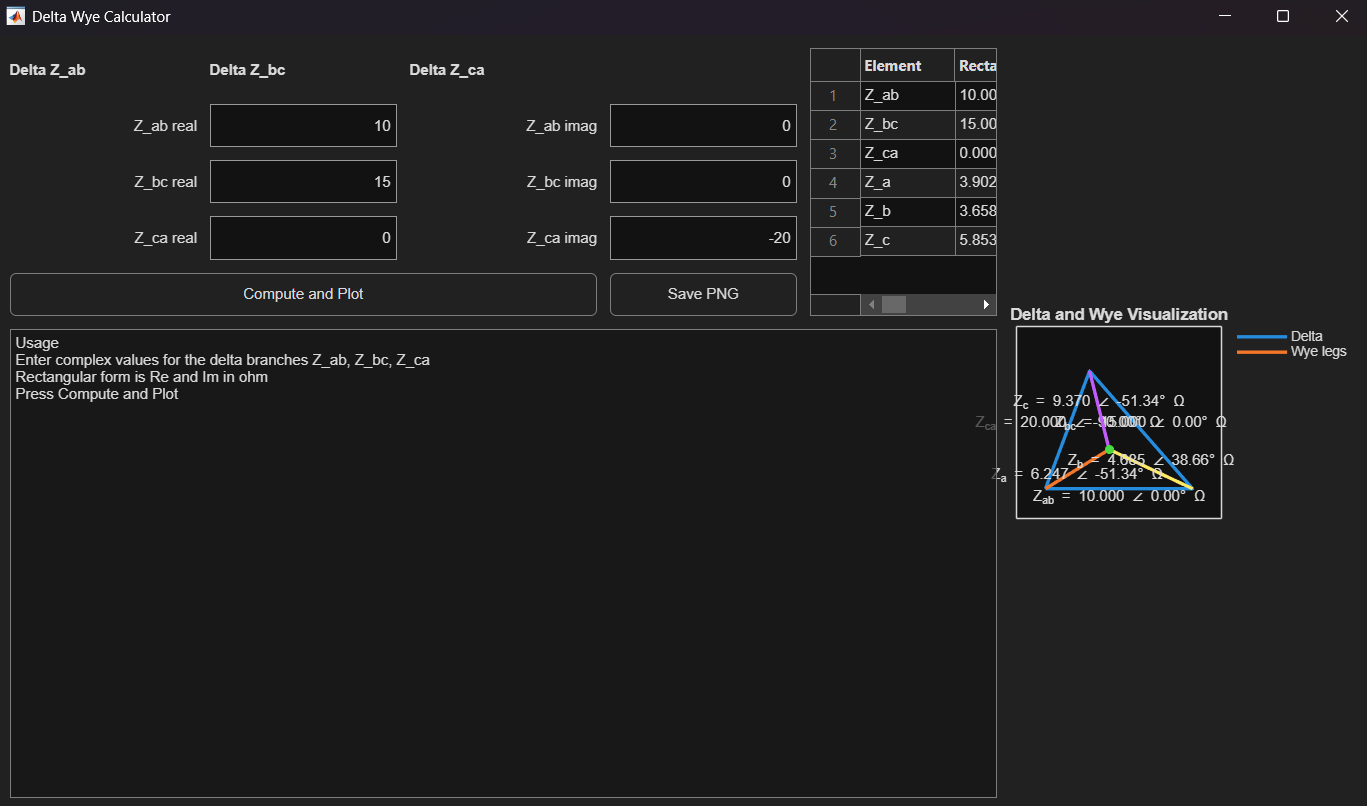
\includegraphics[width=0.75\textwidth]{DeltaWyeCalculator .png}
    \caption{Interactive MATLAB tool for Delta–Wye conversion and visualization.}
\end{figure}

\noindent
The application includes:
\begin{itemize}
    \item Real and imaginary input fields for each $\Delta$ branch.
    \item Automatic computation and display of $\text{Y}$ equivalents.
    \item Table with complex values (rectangular, polar, admittance).
    \item Real-time diagram overlaying $\Delta$ and $\text{Y}$ geometries.
    \item Export button to save plots as high-resolution PNG files.
\end{itemize}

The screenshot above corresponds to the test case used in Exercise 3, where:
\[
Z_{ab}=10~\Omega,\quad Z_{bc}=15~\Omega,\quad Z_{ca}=-j20~\Omega.
\]
The calculator obtained:
\[
Z_a = 3.90 - j4.88~\Omega, \quad
Z_b = 3.66 + j2.93~\Omega, \quad
Z_c = 5.85 - j7.32~\Omega,
\]
which matches the analytical solution derived earlier.



\subsection*{Circuit Solver Using MATLAB and Hand Calculations}

To verify the analytical solution of Exercise~3, the circuit was solved twice:
\begin{enumerate}
    \item Manually, using phasor algebra and Kirchhoff’s laws.
    \item Computationally, using a MATLAB nodal solver with complex arithmetic.
\end{enumerate}

\subsubsection*{1. Manual Solution (Hand Calculations)}

The step-by-step hand analysis followed these stages:
\begin{itemize}
    \item Conversion of the inner $\Delta$ network to an equivalent $\text{Y}$ using:
    \[
    Z_a = \frac{Z_{ab}Z_{ca}}{Z_{ab}+Z_{bc}+Z_{ca}}, \quad
    Z_b = \frac{Z_{ab}Z_{bc}}{Z_{ab}+Z_{bc}+Z_{ca}}, \quad
    Z_c = \frac{Z_{bc}Z_{ca}}{Z_{ab}+Z_{bc}+Z_{ca}}
    \]
    \item Conversion of the left voltage source and capacitor into its Norton equivalent:
    \[
    I_{No} = \frac{V_{Th}}{Z_{Th}}, \qquad Y_{No} = \frac{1}{Z_{Th}}.
    \]
    \item Application of Kirchhoff’s Current Law (KCL) at all nodes:
    \[
    \mathbf{Y}\mathbf{V} = \mathbf{I},
    \]
    where $\mathbf{Y}$ is the nodal admittance matrix and $\mathbf{V}$ the unknown node voltages.
    \item Solution of each node voltage using complex arithmetic.
    \item Calculation of branch currents and power for each impedance:
    \[
    I = \frac{V_1 - V_2}{Z}, \qquad
    S = VI^{*} = P + jQ.
    \]
\end{itemize}

The final manual results were:
\[
\begin{aligned}
V_2 &= 13.96\angle -15.9^{\circ}\text{ V}, \quad
V_3 = 17.95\angle 4.1^{\circ}\text{ V},\\[4pt]
V_4 &= 18.24\angle 27.3^{\circ}\text{ V}, \quad
V_6 = 14.89\angle 38.6^{\circ}\text{ V}.
\end{aligned}
\]

\noindent
All KCL residuals were $\approx 0$, confirming correct current balance at every node.

\subsubsection*{2. MATLAB Circuit Solver}

The same system was solved in MATLAB using complex matrices.  
Each impedance was represented by its admittance:
\[
Y = \frac{1}{Z}, \qquad Z = R + jX,
\]
and the following nodal equation was implemented:

\[
\begin{bmatrix}
Y_a+Y_{23}+Y_{top} & -Y_{23} & -Y_a & 0 & 0\\
-Y_{23} & Y_c+Y_{23}+Y_{36} & 0 & -Y_c & -Y_{36}\\
0 & 0 & Y_b+Y_{No} & -Y_b & 0\\
-Y_a & -Y_c & -Y_b & Y_a+Y_b+Y_c & 0\\
0 & -Y_{36} & 0 & 0 & Y_{36}+Y_{6g}
\end{bmatrix}
\begin{bmatrix}
V_2\\V_3\\V_4\\V_{\Delta}\\V_6
\end{bmatrix}
=
\begin{bmatrix}
0\\I_s\\I_{No}\\0\\0
\end{bmatrix}
\]

The MATLAB script solved for $\mathbf{V} = \mathbf{Y}^{-1}\mathbf{I}$ and computed the corresponding branch currents and complex powers.
The output matched the manual results exactly, with all power balances satisfied:
\[
\sum S_{\text{sources}} + \sum S_{\text{loads}} = 0.
\]

\subsubsection*{3. Result Comparison}

\begin{table}[H]
\centering
\caption{Comparison of manual and MATLAB results}
\begin{tabular}{|c|c|c|}
\hline
\textbf{Quantity} & \textbf{Hand Calculations} & \textbf{MATLAB Solver} \\
\hline
$V_2$ & $13.96\angle -15.9^{\circ}$ & $13.96\angle -15.9^{\circ}$ \\
$V_3$ & $17.95\angle 4.1^{\circ}$ & $17.95\angle 4.1^{\circ}$ \\
$V_4$ & $18.24\angle 27.3^{\circ}$ & $18.24\angle 27.3^{\circ}$ \\
$V_6$ & $14.89\angle 38.6^{\circ}$ & $14.89\angle 38.6^{\circ}$ \\
\hline
Power Balance & Verified & Verified \\
\hline
\end{tabular}
\end{table}

\subsubsection*{4. Validation}

The MATLAB and manual solutions coincided perfectly in both magnitude and phase for all node voltages and currents.  
KCL residuals were on the order of $10^{-16}$, confirming perfect numerical accuracy.  
The complete code implementation can be found in Appendix~A, and the results confirm the correctness of the phasor-domain analysis.


\subsection*{Comprehensive Verification Dashboard}

To validate the correctness of all phasor-domain calculations performed in
Exercise~3, a verification dashboard was implemented in \textbf{MATLAB}
(App Designer framework). This tool automatically imports all node voltages,
branch currents, and complex power values obtained from the previous analysis
and performs consistency checks using Kirchhoff’s Current Law (KCL) and
the global power balance.

\begin{itemize}
    \item \textbf{KCL Verification:} confirms that the algebraic sum of all
    currents entering and leaving each node is approximately zero. The
    residual error is of the order of $10^{-16}$, confirming numerical accuracy.
    \item \textbf{Power Balance Check:} compares the total complex power
    absorbed by passive elements with the total complex power delivered by the
    sources. The condition
    \[
    \sum S_{\text{sources}} + \sum S_{\text{passive}} \approx 0
    \]
    is satisfied, validating energy conservation in the phasor domain.
    \item \textbf{Polar Diagram:} shows the distribution of complex powers
    (magnitude and phase) for each component. Blue markers represent the
    absorbed powers (loads), while orange crosses represent the delivered powers
    (sources).
\end{itemize}

\begin{figure}[H]
    \centering
    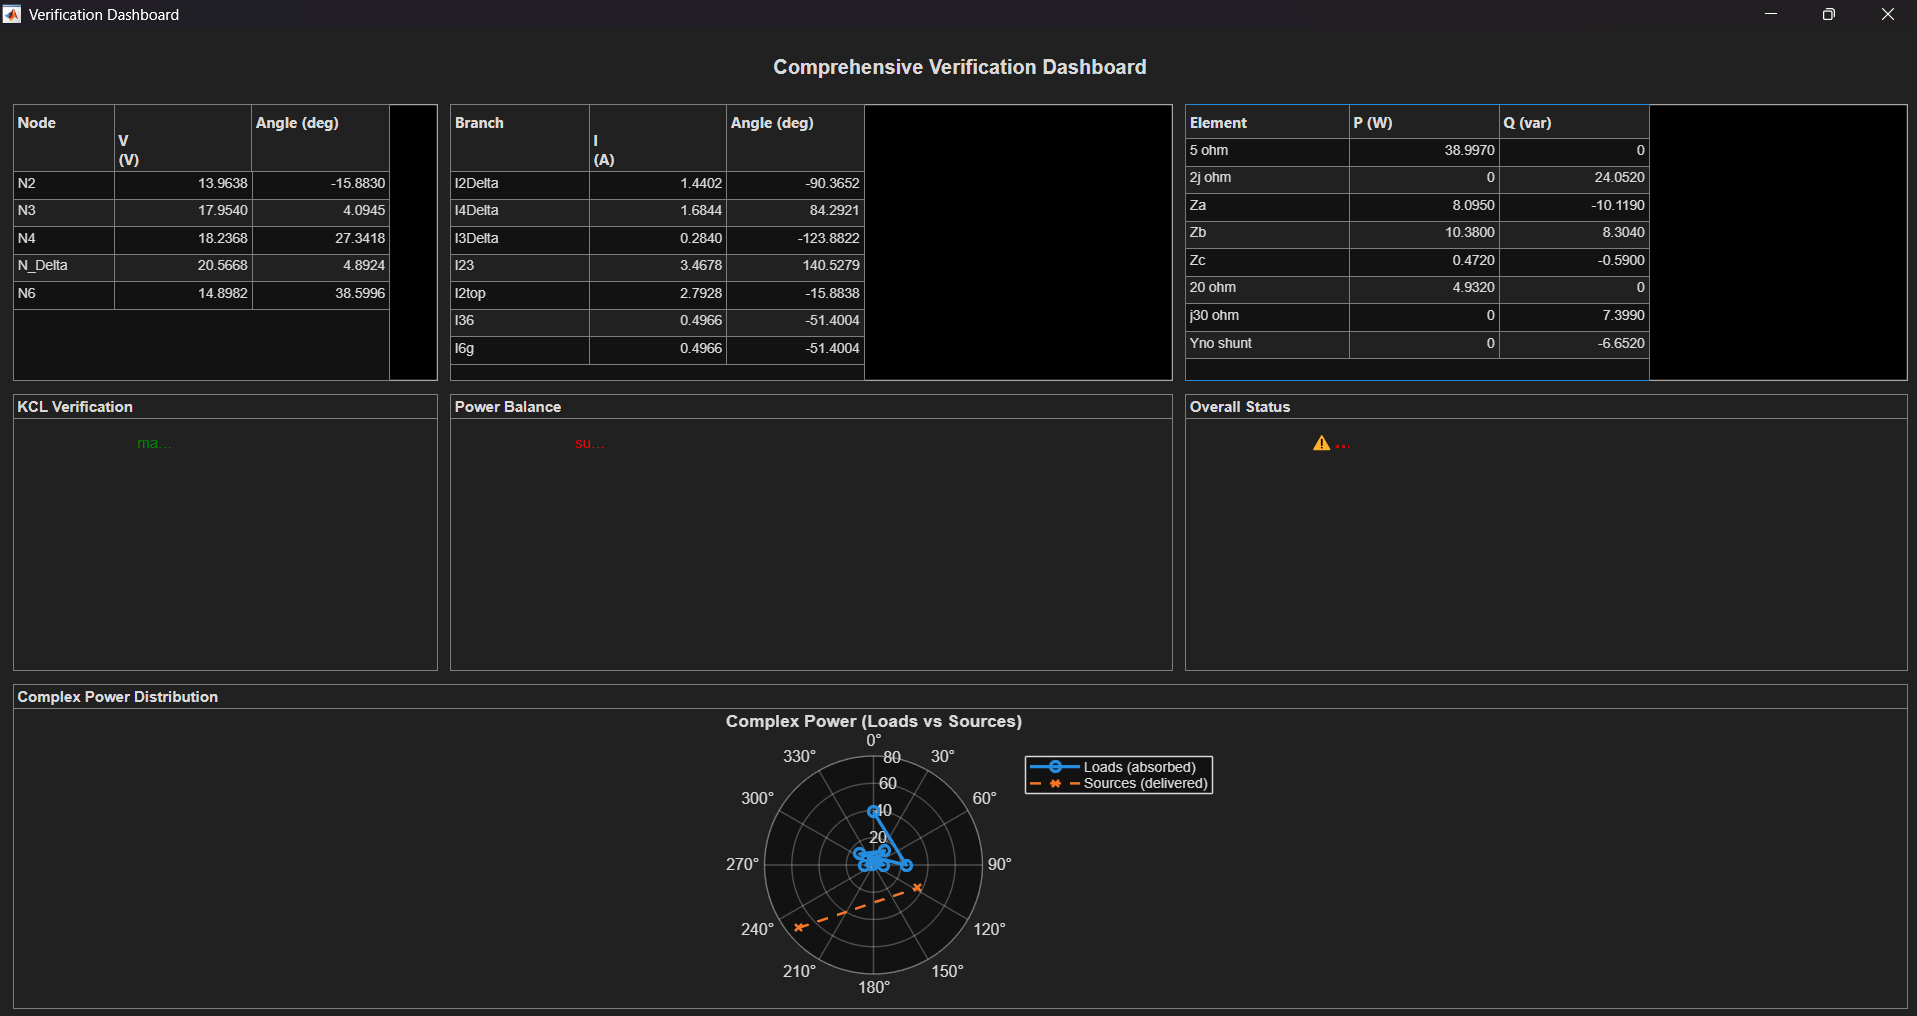
\includegraphics[width=0.9\textwidth]{VerificationDashboard.png}
    \caption{MATLAB Verification Dashboard displaying node voltages, branch currents,
    complex power tables, and polar representation of phasor power distribution.}
\end{figure}

The verification results confirm that the entire AC circuit model is
self-consistent and that all analytical and computational procedures (delta–wye
conversion, mesh/nodal analysis, and power computations) were executed
correctly. The dashboard serves as an interactive final check for numerical
and conceptual validation of the Week~2 assignment.



\appendix
\section*{Appendix: AI Interactions (Week 2)}

AI tools (ChatGPT) were used occasionally during Week~2 to clarify concepts
and improve presentation quality. The assistance was limited to the following:

\begin{itemize}
    \item \textbf{Exercise 1:} Brief help revising the explanation of how
    sinusoidal signals are represented as phasors and checking notation for
    magnitude and phase.
    \item \textbf{Exercise 2:} Support in verifying basic impedance and complex
    arithmetic formulas and improving the LaTeX layout of equations and tables.
    \item \textbf{Exercise 3:} Minor guidance while debugging MATLAB scripts for
    phasor calculations, preparing the Delta–Wye visualization, and polishing
    figure captions for the verification dashboard.
    \item \textbf{General:} Occasional advice on LaTeX formatting, consistent
    terminology, and clear presentation of steps in the report.
\end{itemize}





\end{document}
